\subsection{Теорема о функции, обратной к строго монотонной непрерывной на отрезке функции (функция, обратная к строго монотонной непрерывной на отрезке функции однозначно обратима, строго монотонна и непрерывна).}

\textbf{Теорема.} Пусть $f(x) \in C[a, b]$ и $f(x)$ строго возрастает ($f(x) \uparrow\uparrow$) на $[a, b]$.
Обозначим $A := f(a)$, $B := f(b)$.
Тогда:
\begin{enumerate}
    \item Множество значений $f([a, b]) = [A, B]$.
    \item Обратная функция $x = f^{-1}(y)$ определена и однозначна на $[A, B]$.
    \item $f^{-1}(y) \in C[A, B]$ (непрерывна).
    \item $f^{-1}(y)$ строго возрастает на $[A, B]$.
\end{enumerate}

\begin{tcolorbox}[title=Доказательство]
    \begin{enumerate}
        \item \textbf{Множество значений (включение в одну сторону).}
        Так как $f(x) \uparrow\uparrow$ на $[a, b]$, то:
        \[ \forall x: a \le x \le b \Rightarrow f(a) \le f(x) \le f(b) \Rightarrow A \le f(x) \le B \]
        Следовательно, $f([a, b]) \subset [A, B]$.

        \item \textbf{Множество значений (равенство).}
        По теореме о промежуточном значении (для непрерывной функции):
        \[ \forall C \in [A, B] \;\; \exists c \in [a, b]: f(c) = C \]
        Из п.1 и п.2 следует, что $f([a, b]) = [A, B]$.

        \item \textbf{Существование и однозначность (инъективность).}
        Нужно доказать: $\forall y \in [A, B] \;\; \exists! x \in [a, b]: f(x) = y$.
        Существование доказано в п.2. Докажем единственность от противного.
        Пусть $\exists x', x'' \in [a, b]$ такие, что $x' \neq x''$, но $f(x') = f(x'') = y$.
        Если $x' < x''$, то так как $f(x) \uparrow\uparrow$, должно быть $f(x') < f(x'')$, то есть $y < y$.
        \textbf{Противоречие.} Значит, обратная функция $f^{-1}(y)$ существует на $[A, B]$.

        \item \textbf{Монотонность обратной функции.}
        Докажем, что $f^{-1}(y) \uparrow\uparrow$ на $[A, B]$.
        Пусть $y_1 < y_2$. Обозначим $x_1 = f^{-1}(y_1)$, $x_2 = f^{-1}(y_2)$.
        Предположим противное (что функция не возрастает):
        \begin{enumerate}
            \item Если $x_1 = x_2$, то $f(x_1) = f(x_2) \Rightarrow y_1 = y_2$ (невозможно, так как $y_1 < y_2$).
            \item Если $x_1 > x_2$. Так как $f(x) \uparrow\uparrow$, то $f(x_1) > f(x_2) \Rightarrow y_1 > y_2$.
            \textbf{Противоречие} с условием $y_1 < y_2$.
        \end{enumerate}
        Следовательно, $x_1 < x_2$, то есть $f^{-1}(y)$ строго возрастает.

        \item \textbf{Непрерывность обратной функции.}
        Нужно доказать, что $f^{-1}(y)$ непрерывна в любой точке $y_0 \in [A, B]$.
        Пусть $x_0 = f^{-1}(y_0)$.

        \textbf{а) Внутренняя точка:} $y_0 \in (A, B) \Rightarrow x_0 \in (a, b)$.
        Зафиксируем $\forall \varepsilon > 0$ (такое, что $[x_0 - \varepsilon, x_0 + \varepsilon] \subset [a, b]$).
        Рассмотрим значения функции на концах $\varepsilon$-окрестности:
        \[ y_{-\varepsilon} = f(x_0 - \varepsilon), \quad y_{+\varepsilon} = f(x_0 + \varepsilon) \]
        Так как $f \uparrow\uparrow$, то $y_{-\varepsilon} < y_0 < y_{+\varepsilon}$.
        Выберем $\delta$:
        \[ \delta := \min \{ y_0 - f(x_0 - \varepsilon); \; f(x_0 + \varepsilon) - y_0 \} \]
        Тогда окрестность $(y_0 - \delta, y_0 + \delta)$ целиком лежит внутри $(y_{-\varepsilon}, y_{+\varepsilon})$.
	В силу монотонности обратной функции, все точки из $\delta$-окрестности $y_0$ отобразятся внутрь $\varepsilon$-окрестности $x_0$:
        \[ |y - y_0| < \delta \Rightarrow |f^{-1}(y) - x_0| < \varepsilon \]

	\begin{center}
	\begin{tikzpicture}[scale=1.2]
    % Оси
    \draw[->] (-0.5,0) -- (5,0) node[right] {$x$};
    \draw[->] (0,-0.5) -- (0,4.5) node[above] {$y$};

    % Координаты точек
    \def\xz{2.5}  \def\yz{2.2}   % Точка (x0, y0)
    \def\xl{1.5}  \def\yl{1.2}   % Точка слева (минус эпсилон)
    \def\xr{3.5}  \def\yr{3.5}   % Точка справа (плюс эпсилон)

    % График функции (кривая Безье через эти точки)
    \draw[thick] (0.5, 0.5) .. controls (1.5, 0.8) and (2.5, 2.2) .. (4.2, 4) node[right] {$f(x)$};

    % Проекции для x0, y0
    \draw[dashed] (\xz, 0) -- (\xz, \yz) -- (0, \yz) node[left] {$y_0$};
    \node[below] at (\xz, 0) {$x_0$};

    % Проекции для x0 - epsilon
    \draw[dashed] (\xl, 0) -- (\xl, \yl) -- (0, \yl) node[left] {$f(x_0 - \varepsilon)$};
    \node[below] at (\xl, 0) {$x_0 - \varepsilon$};

    % Проекции для x0 + epsilon
    \draw[dashed] (\xr, 0) -- (\xr, \yr) -- (0, \yr) node[left] {$f(x_0 + \varepsilon)$};
    \node[below] at (\xr, 0) {$x_0 + \varepsilon$};

	\end{tikzpicture}
	\end{center}

        \textbf{б) Граничная точка:} $y_0 = A$ (для $B$ аналогично).
        Тогда $x_0 = a$.
        Берем $\forall \varepsilon > 0$ (такое, что $a + \varepsilon \le b$).
        Рассмотрим $f(a + \varepsilon)$.
        Так как $f$ возрастает, $f(a + \varepsilon) > f(a) = A$.
        Возьмем $\delta = f(a + \varepsilon) - A$.
        Тогда для всех $y \in [A, A + \delta)$:
        \[ A \le y < f(a+\varepsilon) \Rightarrow a \le f^{-1}(y) < a + \varepsilon \]
        Что означает непрерывность справа в точке $A$.
        
        \begin{center}
        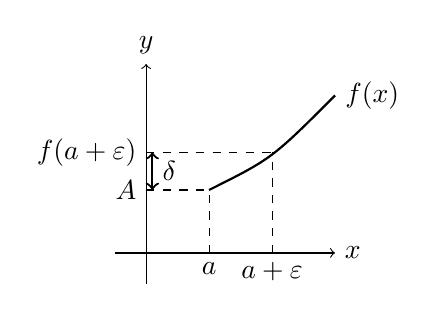
\begin{tikzpicture}[scale=0.8]
            \draw[->] (-0.5,0) -- (3,0) node[right] {$x$};
            \draw[->] (0,-0.5) -- (0,3) node[above] {$y$};
            \draw[thick] (1,1) .. controls (2,1.5) .. (3,2.5) node[right] {$f(x)$};
            
            \draw[dashed] (1,0) node[below] {$a$} -- (1,1);
            \draw[dashed] (2,0) node[below] {$a+\varepsilon$} -- (2,1.6);
            
            \draw[dashed] (0,1) node[left] {$A$} -- (1,1);
            \draw[dashed] (0,1.6) node[left] {$f(a+\varepsilon)$} -- (2,1.6);
            
            \draw[thick, <->] (0.1, 1) -- (0.1, 1.6) node[midway, right] {$\delta$};
        \end{tikzpicture}
        \end{center}
    \end{enumerate}
\end{tcolorbox}
